\documentclass[a4paper,10pt]{article}
\usepackage[utf8x]{inputenc}
\usepackage{graphicx}

%With boxes
%\usepackage{float}
%\floatstyle{boxed} 
%\restylefloat{figure}

%max size of figures
\usepackage[export]{adjustbox}

%Only float in section
\usepackage[section]{placeins}

%landscape in pictures
\usepackage{lscape}

%opening
\title{Generated Metamodel-Evolution Output}
\author{Florian}

\begin{document}

\maketitle

\begin{abstract}

\end{abstract}

\section{Graph TL}

\begin{figure}[h!]
  \centering
    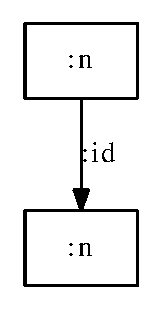
\includegraphics[max size={\textwidth}{\textheight}]{TL}
  \caption{L}
\end{figure}

\section{Graph TK}

\begin{figure}[h!]
  \centering
    
\includegraphics[max size={\textwidth}{\textheight}]{TK}
  \caption{TK}
\end{figure}

\section{Graph TR}

\begin{figure}[h!]
  \centering
    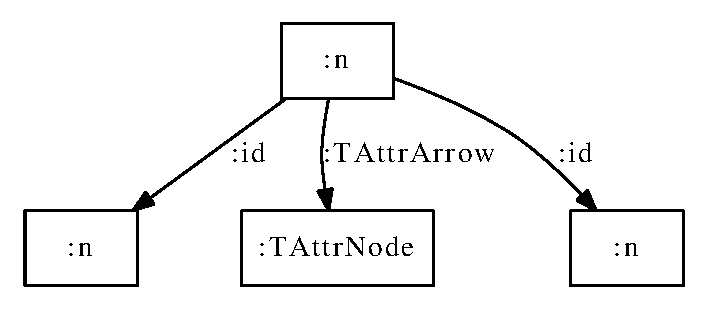
\includegraphics[max size={\textwidth}{\textheight}]{TR}
  \caption{TR}
\end{figure}

\section{Graph TG}

\begin{figure}[h!]
  \centering
    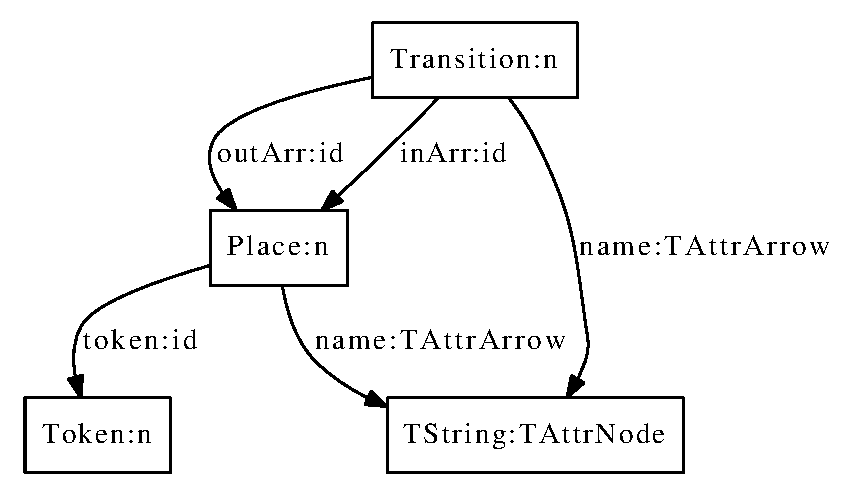
\includegraphics[max size={\textwidth}{\textheight}]{TG}
  \caption{TG}
\end{figure}

\section{Graph TC}

\begin{figure}[h!]
  \centering
    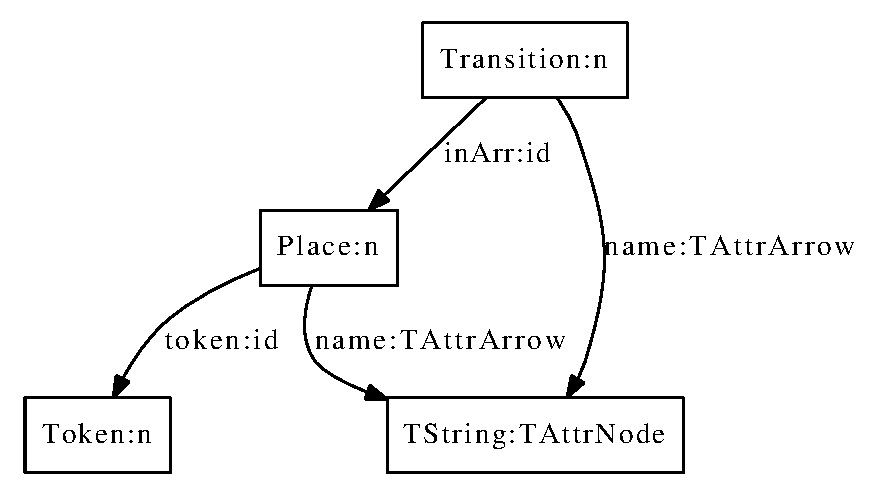
\includegraphics[max size={\textwidth}{\textheight}]{TC}
  \caption{TC}
\end{figure}


\section{Graph TH}

\begin{figure}[h!]
  \centering
    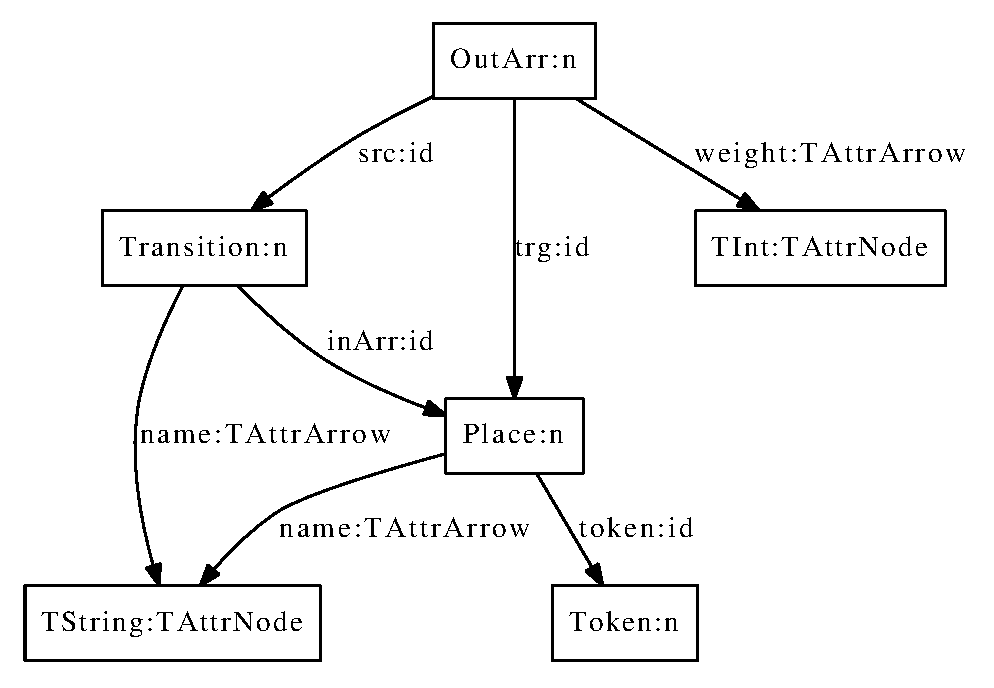
\includegraphics[max size={\textwidth}{\textheight}]{TH}
  \caption{TH}
\end{figure}


\section{Graph L}

\begin{figure}[h!]
  \centering
    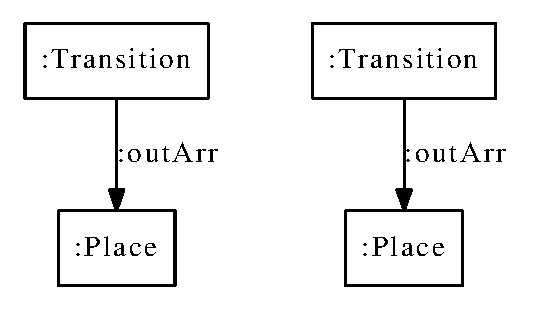
\includegraphics[max size={\textwidth}{\textheight}]{L}
  \caption{L}
\end{figure}

\section{Graph K}

\begin{figure}[h!]
  \centering
    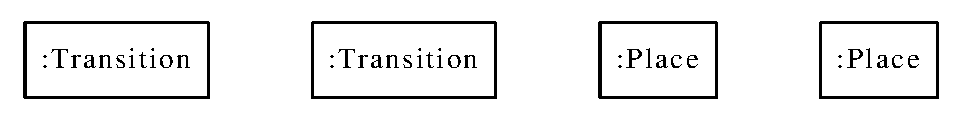
\includegraphics[max size={\textwidth}{\textheight}]{K}
  \caption{K}
\end{figure}

\section{Graph R}

\begin{figure}[h!]
  \centering
    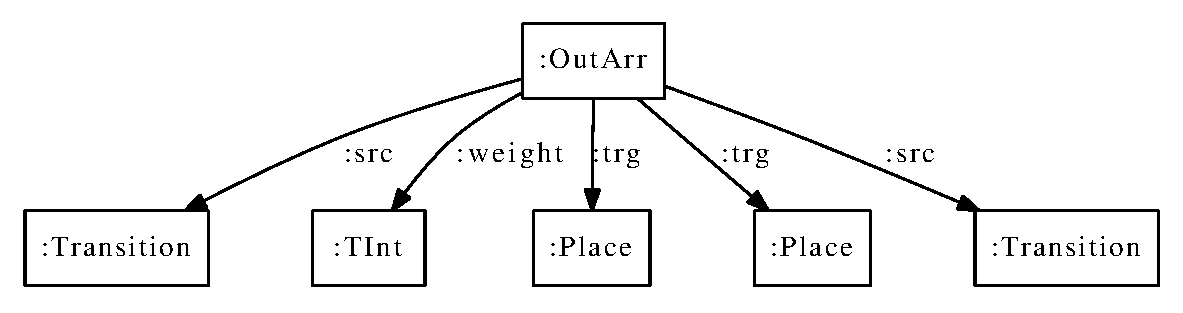
\includegraphics[max size={\textwidth}{\textheight}]{R}
  \caption{R}
\end{figure}

\section{Graph G}

\begin{figure}[h!]
  \centering
    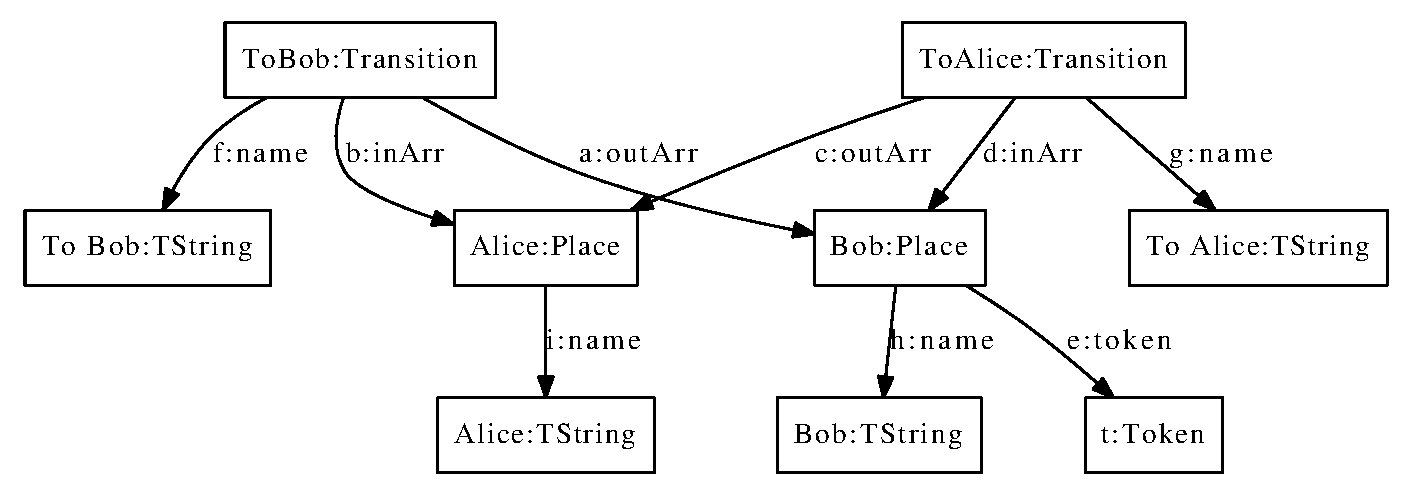
\includegraphics[max size={\textwidth}{\textheight}]{G}
  \caption{G}
\end{figure}

\section{Graph C}

\begin{figure}[h!]
  \centering
    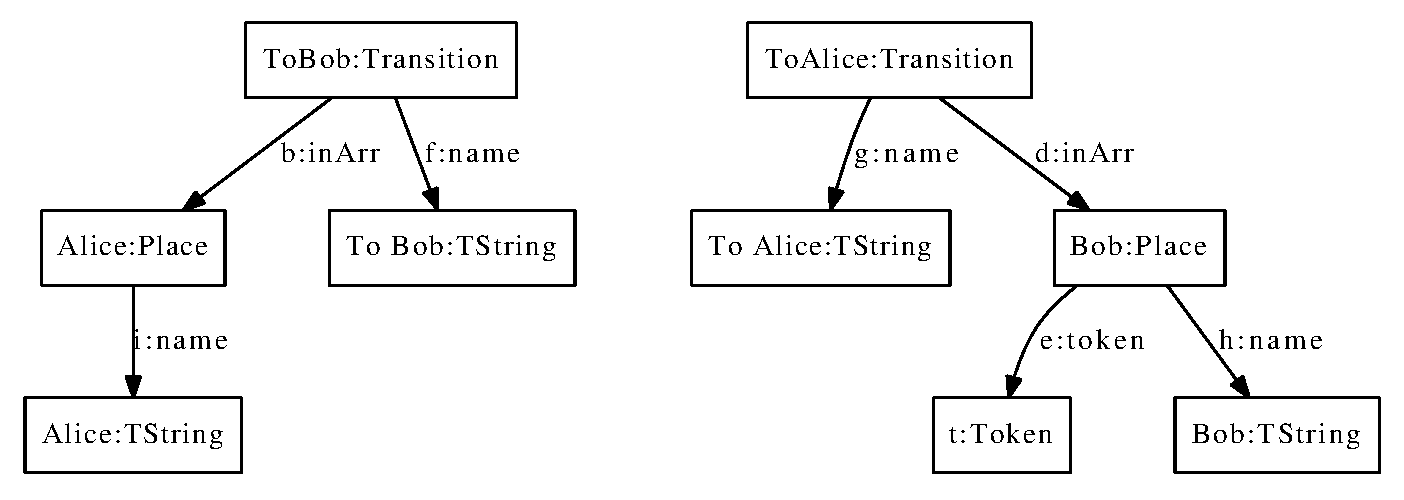
\includegraphics[max size={\textwidth}{\textheight}]{C}
  \caption{C}
\end{figure}


\section{Graph H}

\begin{figure}[h!]
  \centering
    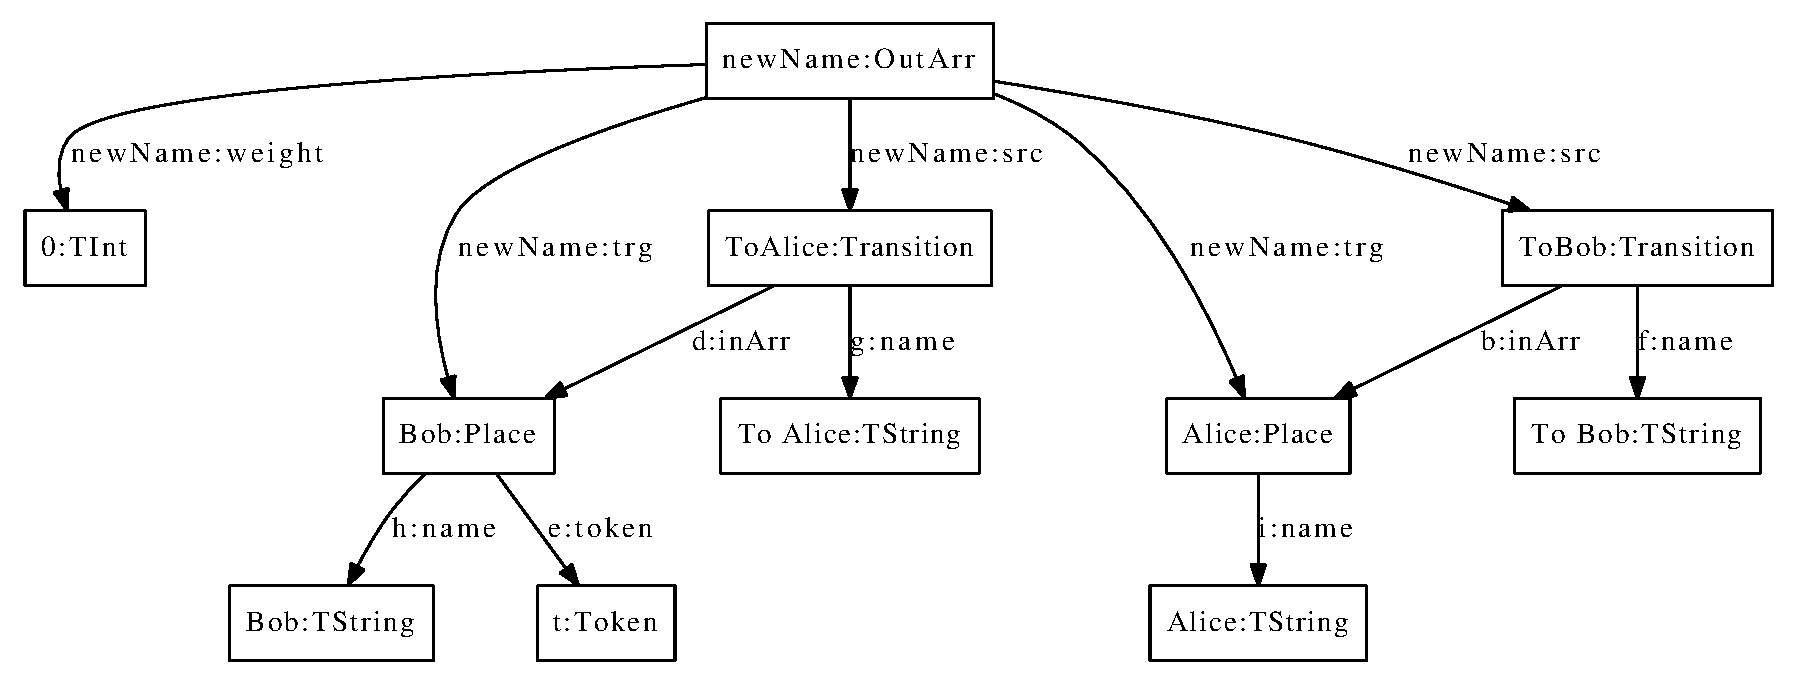
\includegraphics[max size={\textwidth}{\textheight}]{H}
  \caption{H}
\end{figure}


\begin{landscape}

\section{Double-Cube Top}
\begin{figure}[ht]
\begin{minipage}[b]{0.33\linewidth}
\centering
   \fbox{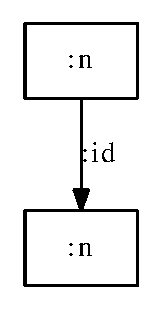
\includegraphics[max size={0.9\textwidth}{0.9\textheight}]{TL}}
\caption{TL}
\label{fig:figure1}
\end{minipage}
\hspace{0.5cm}
\begin{minipage}[b]{0.33\linewidth}
\centering
   \fbox{
\includegraphics[max size={0.9\textwidth}{0.9\textheight}]{TK}}
\caption{TK}
\label{fig:figure2}
\end{minipage}
\begin{minipage}[b]{0.33\linewidth}
\centering
   \fbox{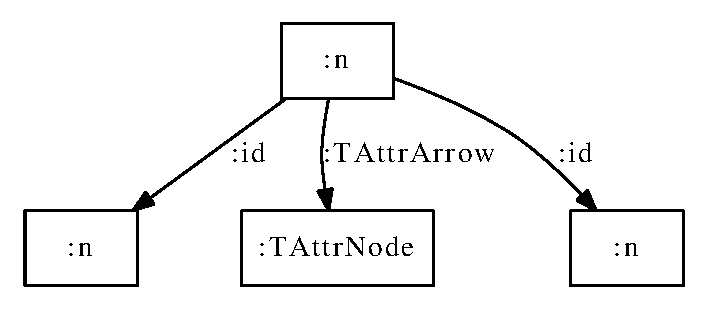
\includegraphics[max size={0.9\textwidth}{0.9\textheight}]{TR}}
\caption{TR}
\label{fig:figure1}
\end{minipage}
\begin{minipage}[b]{0.33\linewidth}
\centering
   \fbox{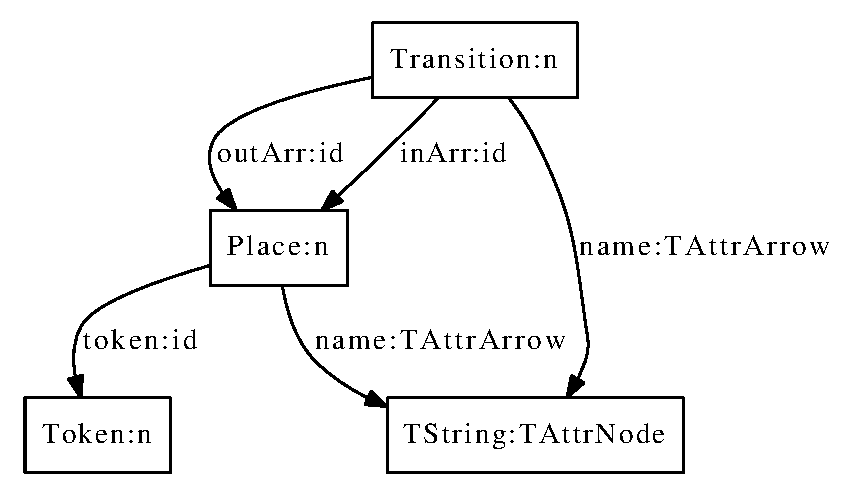
\includegraphics[max size={0.9\textwidth}{0.9\textheight}]{TG}}
\caption{TG}
\label{fig:figure1}
\end{minipage}
\hspace{0.5cm}
\begin{minipage}[b]{0.33\linewidth}
\centering
   \fbox{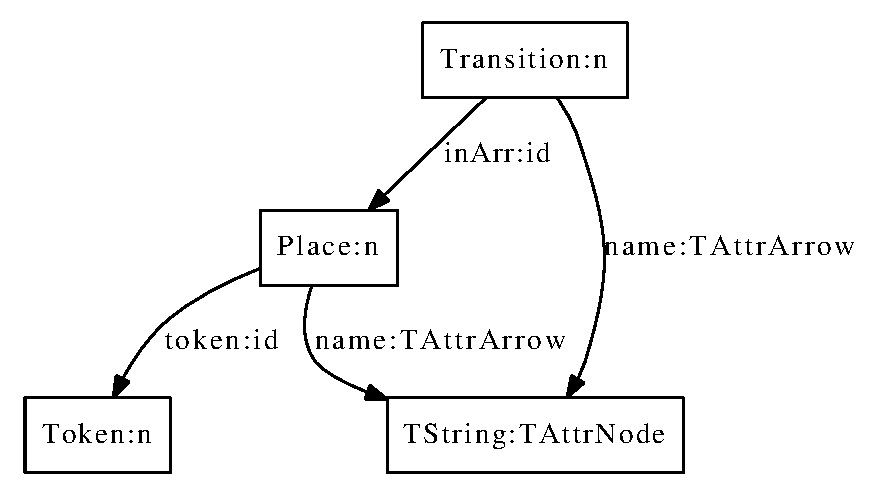
\includegraphics[max size={0.9\textwidth}{0.9\textheight}]{TC}}
\caption{TC}
\label{fig:figure2}
\end{minipage}
\begin{minipage}[b]{0.33\linewidth}
\centering
   \fbox{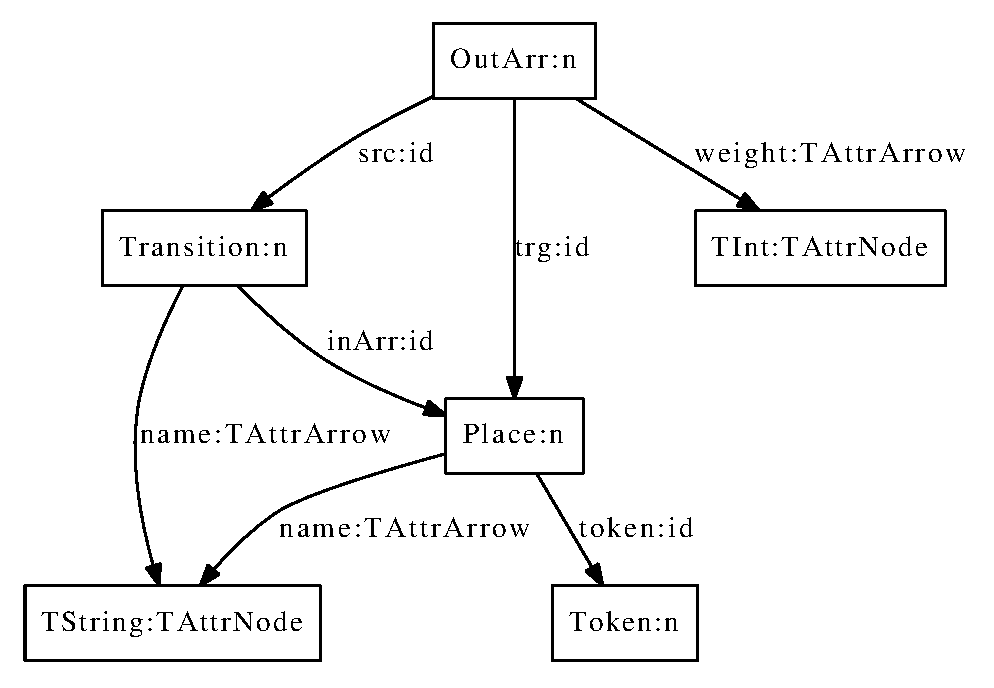
\includegraphics[max size={0.9\textwidth}{0.9\textheight}]{TH}}
\caption{TH}
\label{fig:figure1}
\end{minipage}
\end{figure}


\section{Double-Cube Bottom}

\begin{figure}[ht]
\begin{minipage}[b]{0.33\linewidth}
\centering
   \fbox{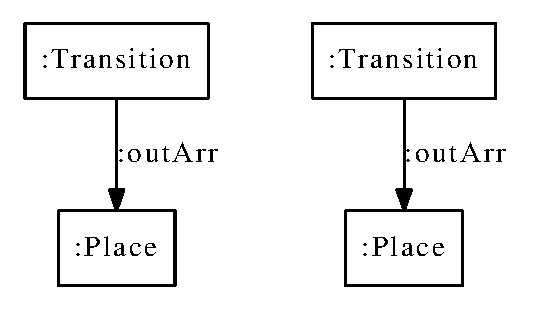
\includegraphics[max size={0.9\textwidth}{0.9\textheight}]{L}}
\caption{L}
\label{fig:figure1}
\end{minipage}
\hspace{0.5cm}
\begin{minipage}[b]{0.33\linewidth}
\centering
   \fbox{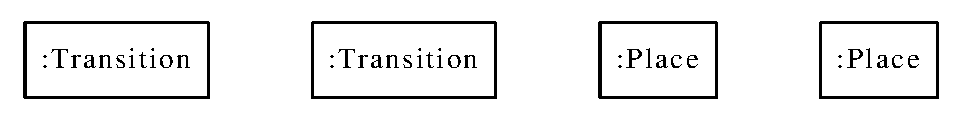
\includegraphics[max size={0.9\textwidth}{0.9\textheight}]{K}}
\caption{K}
\label{fig:figure2}
\end{minipage}
\begin{minipage}[b]{0.33\linewidth}
\centering
   \fbox{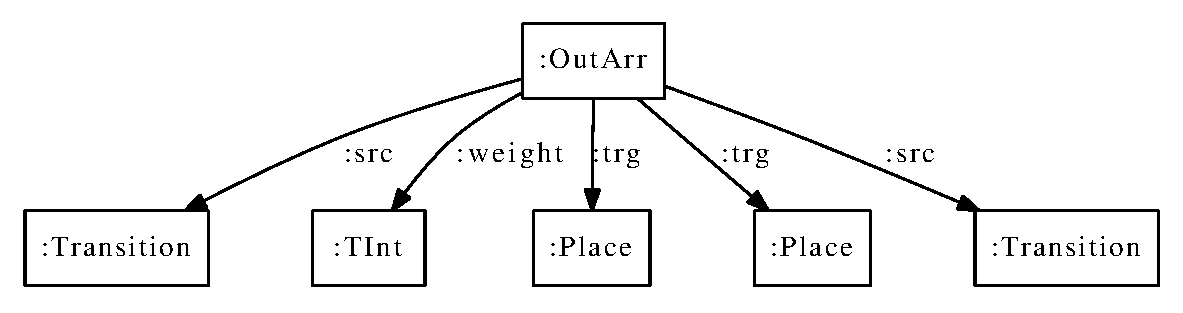
\includegraphics[max size={0.9\textwidth}{0.9\textheight}]{R}}
\caption{R}
\label{fig:figure1}
\end{minipage}
\begin{minipage}[b]{0.33\linewidth}
\centering
   \fbox{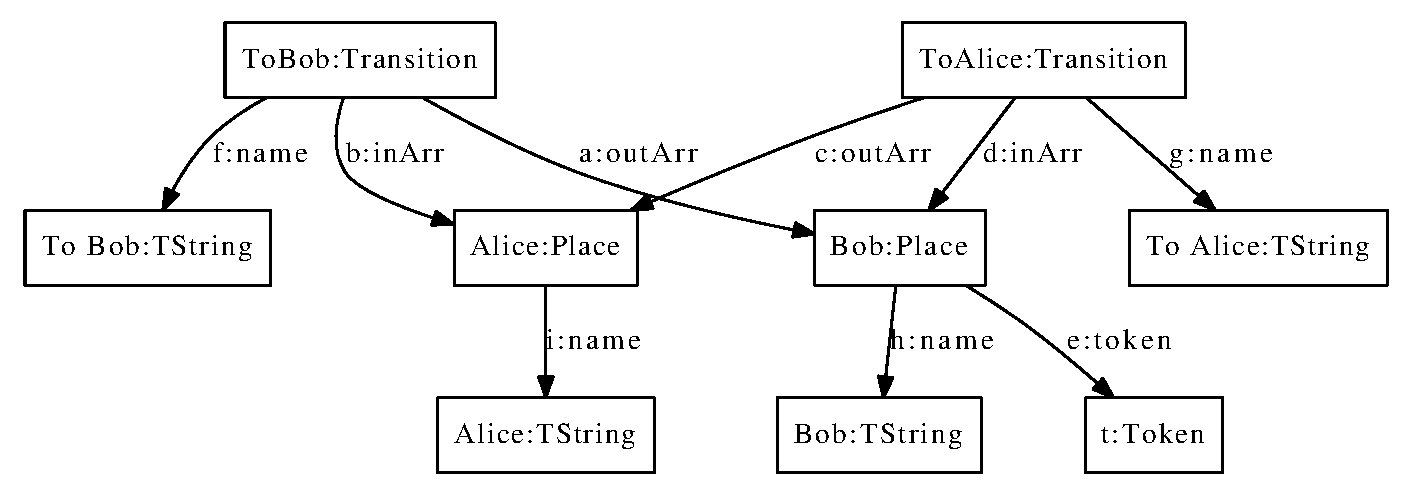
\includegraphics[max size={0.9\textwidth}{0.9\textheight}]{G}}
\caption{G}
\label{fig:figure1}
\end{minipage}
\hspace{0.5cm}
\begin{minipage}[b]{0.33\linewidth}
\centering
   \fbox{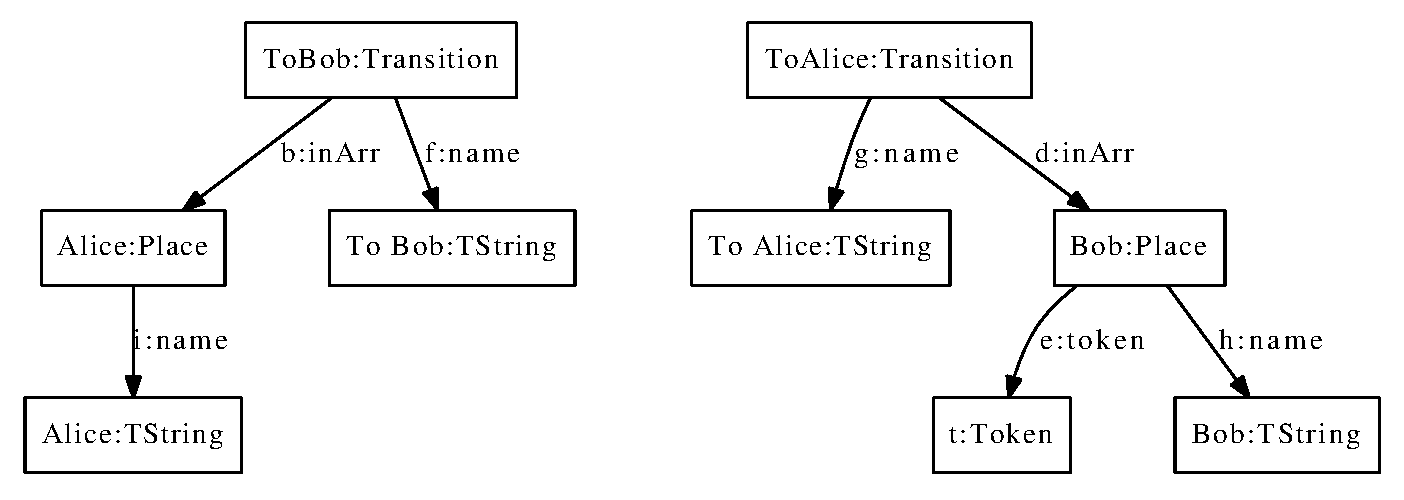
\includegraphics[max size={0.9\textwidth}{0.9\textheight}]{C}}
\caption{C}
\label{fig:figure2}
\end{minipage}
\begin{minipage}[b]{0.33\linewidth}
\centering
   \fbox{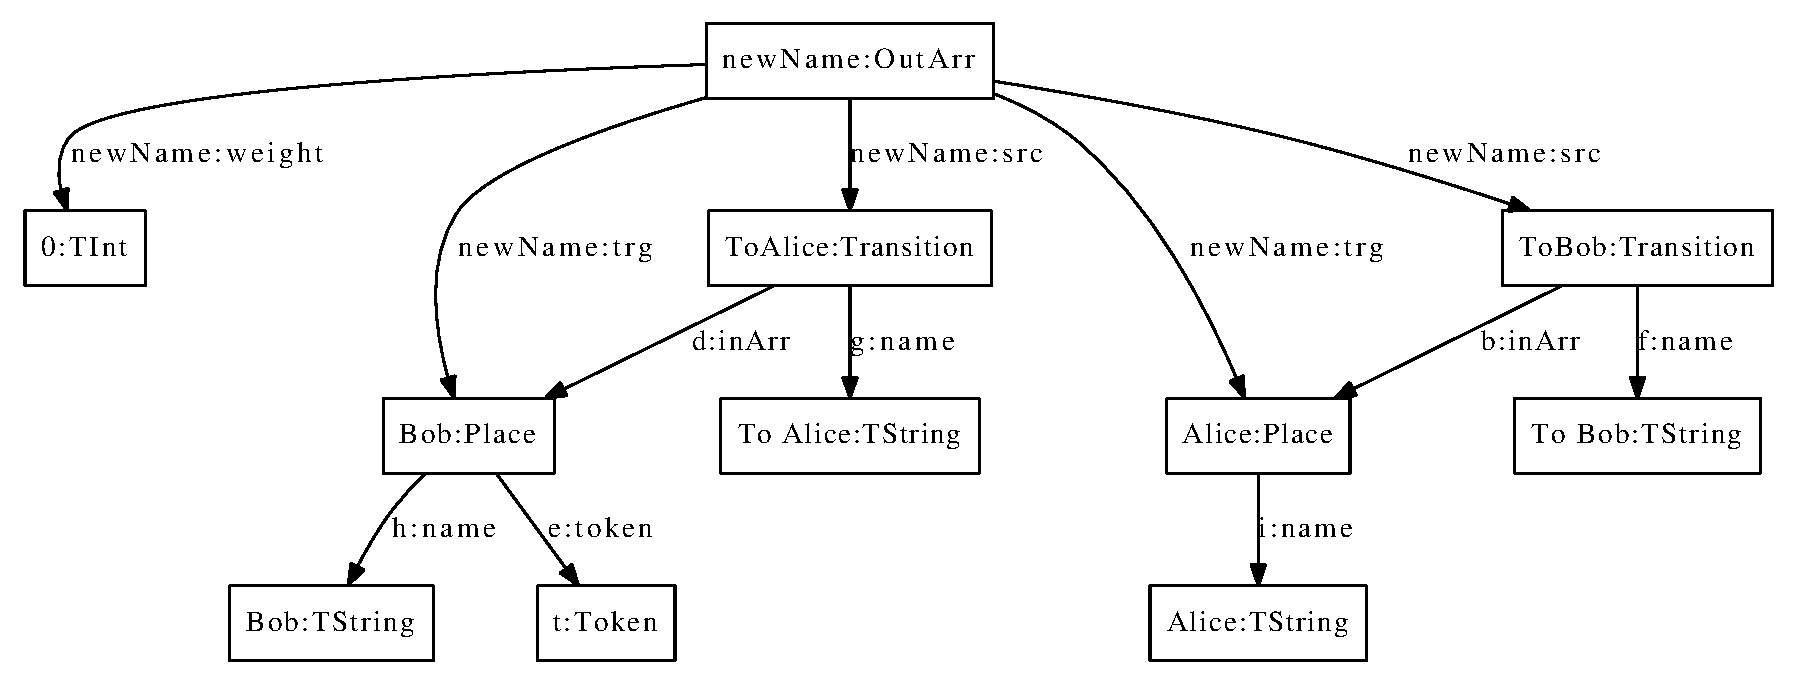
\includegraphics[max size={0.9\textwidth}{0.9\textheight}]{H}}
\caption{H}
\label{fig:figure1}
\end{minipage}
\end{figure}

\end{landscape}
\end{document} 
